\documentclass[tikz,border=12pt]{standalone}
\usepackage[T1]{fontenc}
\usepackage{tikz}
\usetikzlibrary{positioning,arrows.meta,fit,backgrounds,calc}

\definecolor{fglight}{HTML}{e5e5e5}
\definecolor{accent}{HTML}{60a5fa}
\definecolor{muted}{HTML}{999999}
\definecolor{nixblue}{HTML}{7eb8da}
\definecolor{rustred}{HTML}{dea584}
\definecolor{boxbg}{HTML}{2a2a2a}
\definecolor{cachgreen}{HTML}{34d399}

\begin{document}
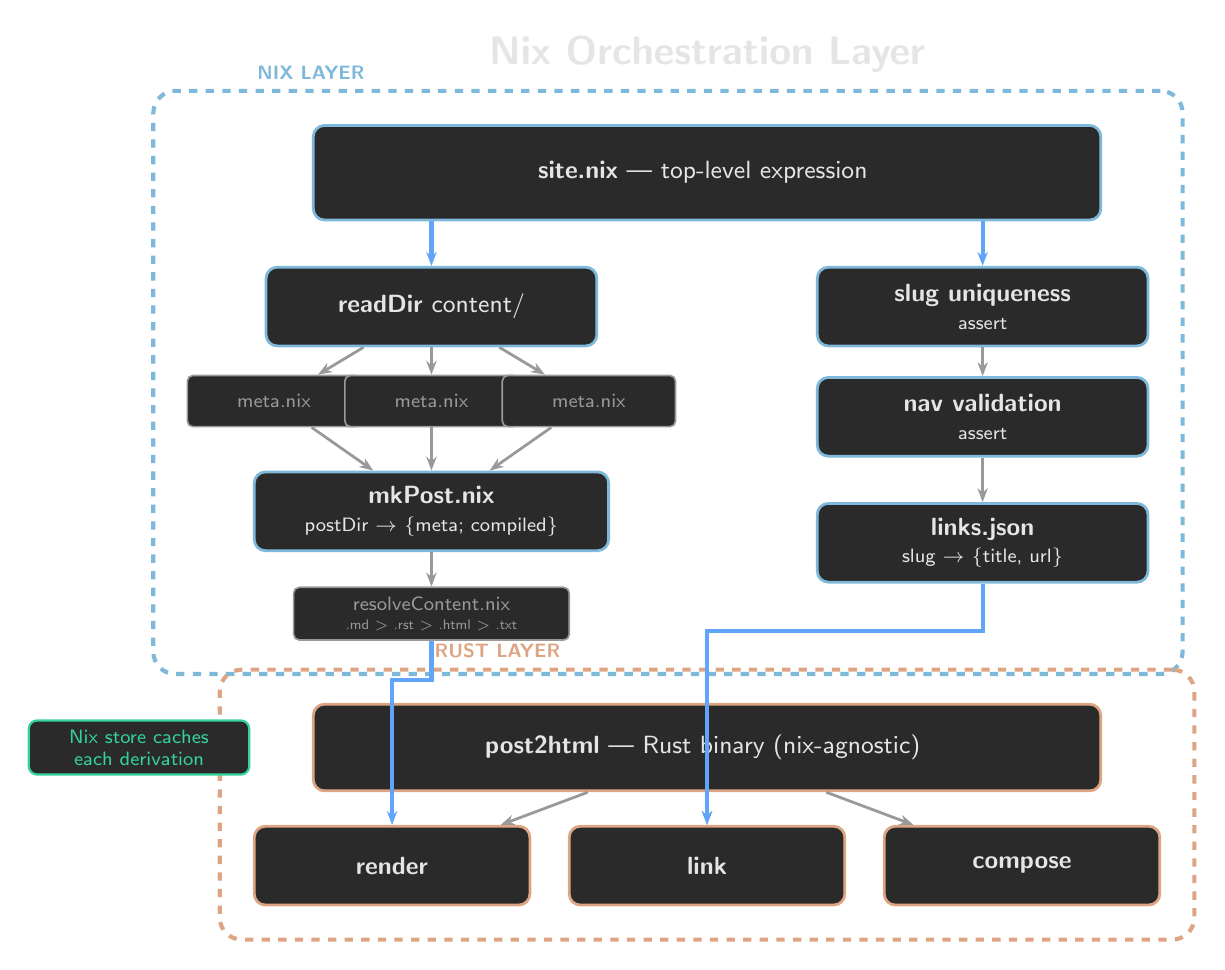
\begin{tikzpicture}[
    >={Stealth[length=5pt]},
    every node/.style={font=\sffamily},
    nixbox/.style={
        rounded corners=4pt,
        minimum width=4.2cm,
        minimum height=1cm,
        align=center,
        text=fglight,
        draw=nixblue,
        line width=1pt,
        fill=boxbg,
        font=\sffamily\small,
    },
    rustbox/.style={
        rounded corners=4pt,
        minimum width=3.5cm,
        minimum height=1cm,
        align=center,
        text=fglight,
        draw=rustred,
        line width=1pt,
        fill=boxbg,
        font=\sffamily\small,
    },
    filebox/.style={
        rounded corners=2pt,
        minimum width=2.2cm,
        minimum height=0.65cm,
        align=center,
        text=muted,
        draw=muted,
        line width=0.6pt,
        fill=boxbg,
        font=\sffamily\scriptsize,
    },
    arr/.style={->,line width=1pt,color=muted},
    thickarr/.style={->,line width=1.5pt,color=accent},
    note/.style={font=\sffamily\tiny,text=muted,align=left},
]

% === Title ===
\node[font=\sffamily\Large\bfseries,text=fglight] at (0,10) {Nix Orchestration Layer};

% === site.nix ===
\node[nixbox,minimum width=10cm,minimum height=1.2cm] (site) at (0,8.5) {
    \textbf{site.nix} --- top-level expression
};

% === Left: content discovery ===
\node[nixbox] (discover) at (-3.5,6.8) {\textbf{readDir} content/};

\node[filebox] (m1) at (-5.5,5.6) {meta.nix};
\node[filebox] (m2) at (-3.5,5.6) {meta.nix};
\node[filebox] (m3) at (-1.5,5.6) {meta.nix};

\node[nixbox,minimum width=4.5cm] (mkpost) at (-3.5,4.2) {
    \textbf{mkPost.nix}\\[-1pt]
    {\scriptsize postDir $\to$ \{meta; compiled\}}
};

\node[filebox,minimum width=3.5cm] (resolve) at (-3.5,2.9) {
    resolveContent.nix\\[-1pt]
    {\tiny .md $>$ .rst $>$ .html $>$ .txt}
};

% === Right: validation + registry ===
\node[nixbox] (slugcheck) at (3.5,6.8) {
    \textbf{slug uniqueness}\\[-1pt]
    {\scriptsize assert}
};
\node[nixbox] (navcheck) at (3.5,5.4) {
    \textbf{nav validation}\\[-1pt]
    {\scriptsize assert}
};
\node[nixbox] (links) at (3.5,3.8) {
    \textbf{links.json}\\[-1pt]
    {\scriptsize slug $\to$ \{title, url\}}
};

% === Arrows: Nix layer ===
\draw[thickarr] (site.south -| discover.north) -- (discover.north);
\draw[thickarr] (site.south -| slugcheck.north) -- (slugcheck.north);

\draw[arr] (discover) -- (m1);
\draw[arr] (discover) -- (m2);
\draw[arr] (discover) -- (m3);

\draw[arr] (m1) -- (mkpost);
\draw[arr] (m2) -- (mkpost);
\draw[arr] (m3) -- (mkpost);

\draw[arr] (mkpost) -- (resolve);

\draw[arr] (slugcheck) -- (navcheck);
\draw[arr] (navcheck) -- (links);

% === Rust binary ===
\node[rustbox,minimum width=10cm,minimum height=1.1cm] (binary) at (0,1.2) {
    \textbf{post2html} --- Rust binary (nix-agnostic)
};

\node[rustbox] (render) at (-4,-.3) {\textbf{render}};
\node[rustbox] (link) at (0,-.3) {\textbf{link}};
\node[rustbox] (compose) at (4,-.3) {\textbf{compose}};

\draw[arr] (binary) -- (render);
\draw[arr] (binary) -- (link);
\draw[arr] (binary) -- (compose);

% === Cross-layer arrows ===
\draw[thickarr] (resolve.south) -- ++(0,-0.5) -| (render.north);
\draw[thickarr] (links.south) -- ++(0,-0.6) -| (link.north);

% === Caching note ===
\node[
    rounded corners=3pt,
    draw=cachgreen,
    line width=0.8pt,
    fill=boxbg,
    text=cachgreen,
    font=\sffamily\scriptsize,
    align=center,
    minimum width=2.8cm,
    anchor=east,
] at (-5.8,1.2) {Nix store caches\\each derivation};

% === Region boxes ===
\begin{scope}[on background layer]
    \node[
        rounded corners=8pt,
        draw=nixblue,
        line width=1.5pt,
        dashed,
        inner sep=12pt,
        fit=(site)(discover)(m1)(m3)(mkpost)(resolve)(slugcheck)(navcheck)(links),
        label={[font=\sffamily\scriptsize\bfseries,text=nixblue]above left:NIX LAYER},
    ] {};
    \node[
        rounded corners=8pt,
        draw=rustred,
        line width=1.5pt,
        dashed,
        inner sep=12pt,
        fit=(binary)(render)(link)(compose),
        label={[font=\sffamily\scriptsize\bfseries,text=rustred]above left:RUST LAYER},
    ] {};
\end{scope}

\end{tikzpicture}
\end{document}
